\documentclass[tikz,border=10pt]{standalone}
\usepackage{tikz}
\usetikzlibrary{positioning, fit, calc, shapes.geometric, arrows.meta, backgrounds}

% Define colors from MLSysBook palette
\definecolor{emeraldpine}{HTML}{1A4D3E}
\definecolor{harvardcrimson}{HTML}{A51C30}
\definecolor{ethdarkblue}{HTML}{1F407A}
\definecolor{ethpetrol}{HTML}{007A87}
\definecolor{ethbronze}{HTML}{B87333}
\definecolor{ethpurple}{HTML}{5B4B8A}
\definecolor{ink}{HTML}{1A202C}
\definecolor{softink}{HTML}{4A5568}
\definecolor{paleink}{HTML}{A0AEC0}
\definecolor{cardbg}{HTML}{F8FAFC}
\definecolor{shadecolor}{HTML}{F4F6F9}

% Lighter shades for backgrounds
\colorlet{mpubg}{ethdarkblue!5}
\colorlet{mpuborder}{ethdarkblue!30}
\colorlet{mcubg}{emeraldpine!5}
\colorlet{mcuborder}{emeraldpine!40}
\colorlet{plantbg}{harvardcrimson!5}
\colorlet{plantborder}{harvardcrimson!30}
\colorlet{mailboxbg}{shadecolor}
\colorlet{mailboxborder}{paleink}

\begin{document}
\sffamily
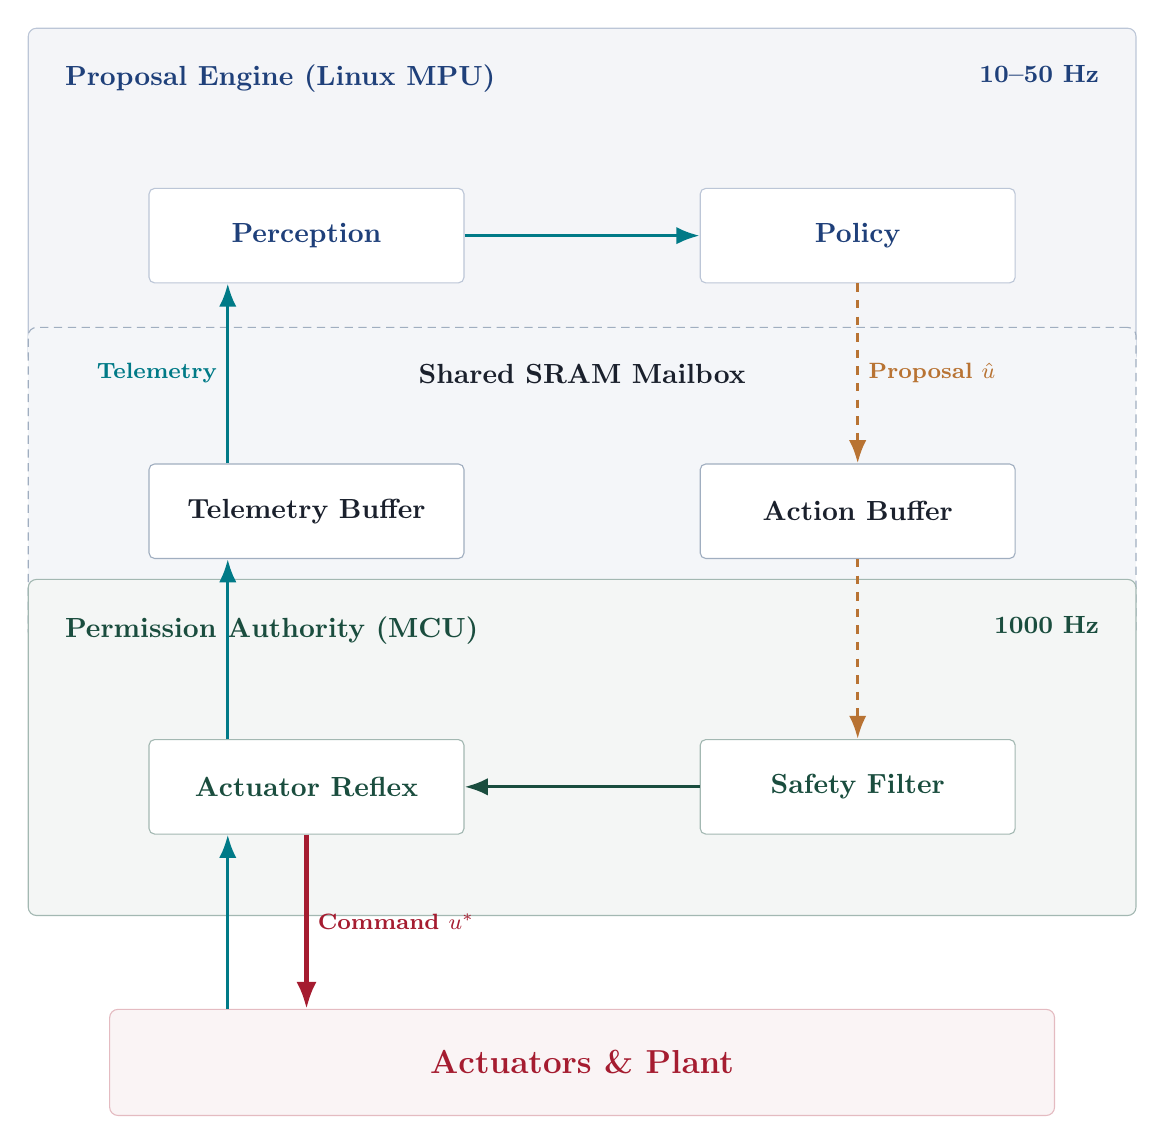
\begin{tikzpicture}[
    >=Latex,
    node distance=1.5cm,
    tier/.style={draw, rounded corners=3pt, inner sep=15pt},
    subcard/.style={draw, rounded corners=2pt, fill=white, minimum height=1.2cm, minimum width=4cm, align=center, font=\bfseries},
    tierhdr/.style={font=\bfseries, anchor=north west},
    cadence/.style={font=\bfseries\small, anchor=north east},
    flowlbl/.style={font=\bfseries\footnotesize, align=center},
    arr_prop/.style={->, draw=ethbronze, line width=1.2pt},
    arr_prop_dashed/.style={->, draw=ethbronze, line width=1.2pt, dashed},
    arr_data/.style={->, draw=ethpetrol, line width=1.2pt},
    arr_cmd/.style={->, draw=harvardcrimson, line width=1.5pt},
    box_telem/.style={subcard, draw=mailboxborder, text=ink},
    box_mpu/.style={subcard, text=ethdarkblue, draw=mpuborder},
    box_mcu/.style={subcard, text=emeraldpine, draw=mcuborder}
]

    % Coordinates for alignment
    \def\colL{0}
    \def\colR{7}
    \def\rowMPU{0}
    \def\rowMB{-3.5}
    \def\rowMCU{-7}
    \def\rowPLANT{-10.5}

    % ----------------------------------------------------
    % NODES
    % ----------------------------------------------------
    
    % TIER 1: MPU
    \node[box_mpu] (perception) at (\colL, \rowMPU) {Perception};
    \node[box_mpu] (policy)     at (\colR, \rowMPU) {Policy};
    
    % TIER 2: MAILBOX
    \node[box_telem] (telembuf) at (\colL, \rowMB) {Telemetry Buffer};
    \node[box_telem] (actbuf)   at (\colR, \rowMB) {Action Buffer};
    
    % TIER 3: MCU
    \node[box_mcu] (reflex)     at (\colL, \rowMCU) {Actuator Reflex};
    \node[box_mcu] (filter)     at (\colR, \rowMCU) {Safety Filter};
    
    % TIER 4: PLANT
    \node[tier, fill=plantbg, draw=plantborder, font=\bfseries\large, text=harvardcrimson, minimum width=12cm, minimum height=1.2cm] (plant) at (3.5, \rowPLANT) {Actuators \& Plant};

    % ----------------------------------------------------
    % BACKGROUND TIERS
    % ----------------------------------------------------
    \begin{scope}[on background layer]
        % MPU Background
        \node[tier, fill=mpubg, draw=mpuborder, fit={(perception) (policy) ($(perception.north west)+(-1,1.5)$) ($(policy.south east)+(1,-0.5)$)}] (tier1) {};
        
        % Mailbox Background
        \node[tier, fill=mailboxbg, draw=mailboxborder, densely dashed, fit={(telembuf) (actbuf) ($(telembuf.north west)+(-1,1.2)$) ($(actbuf.south east)+(1,-0.5)$)}] (tier2) {};
        
        % MCU Background
        \node[tier, fill=mcubg, draw=mcuborder, fit={(reflex) (filter) ($(reflex.north west)+(-1,1.5)$) ($(filter.south east)+(1,-0.5)$)}] (tier3) {};
    \end{scope}

    % Tier Labels
    \node[tierhdr, text=ethdarkblue] at (tier1.north west) [xshift=10pt, yshift=-10pt] {Proposal Engine (Linux MPU)};
    \node[cadence, text=ethdarkblue] at (tier1.north east) [xshift=-10pt, yshift=-10pt] {10--50 Hz};

    \node[tierhdr, text=ink, anchor=north] at (tier2.north) [yshift=-10pt] {Shared SRAM Mailbox};

    \node[tierhdr, text=emeraldpine] at (tier3.north west) [xshift=10pt, yshift=-10pt] {Permission Authority (MCU)};
    \node[cadence, text=emeraldpine] at (tier3.north east) [xshift=-10pt, yshift=-10pt] {1000 Hz};

    % ----------------------------------------------------
    % FLOWS (ARROWS)
    % ----------------------------------------------------
    
    % Horizontal
    \draw[arr_data] (perception) -- (policy);
    \draw[arr_data, draw=emeraldpine] (filter) -- (reflex); % Safety Filter to Reflex is inside MCU
    
    % Vertical Down: Proposals
    \draw[arr_prop_dashed] (policy) -- node[right, flowlbl, text=ethbronze] {Proposal $\hat{u}$} (actbuf);
    \draw[arr_prop_dashed] (actbuf) -- (filter);
    
    % Vertical Down: Command
    \draw[arr_cmd] (reflex) -- node[right, flowlbl, text=harvardcrimson] {Command $u^*$} (reflex |- plant.north);
    
    % Vertical Up: Telemetry
    % To avoid lines passing through text or nodes perfectly centered, we shift the Telemetry line slightly left
    \draw[arr_data] ([xshift=-1cm]reflex |- plant.north) -- ([xshift=-1cm]reflex.south);
    \draw[arr_data] ([xshift=-1cm]reflex.north) -- ([xshift=-1cm]telembuf.south);
    \draw[arr_data] ([xshift=-1cm]telembuf.north) -- node[left, flowlbl, text=ethpetrol] {Telemetry} ([xshift=-1cm]perception.south);

\end{tikzpicture}
\end{document}
